%
% teil1.tex -- Beispiel-File für das Paper
%
% (c) 2020 Prof Dr Andreas Müller, Hochschule Rapperswil
%
% !TEX root = ../../buch.tex
% !TEX encoding = UTF-8
%
\section{Approximative geradlinige Bewegung
\label{geradlinig:section:approximative_geradlinig}}
\kopfrechts{Approximative geradlinige Bewegung}
Der erste approximativ geradlinige Mechanismus war derjenige von James Watt.
In Abbildung~\ref{fig:watts_link} ist der Mechanismus vereinfacht 
dargestellt.
\begin{figure}
    \centering
    \begin{minipage}[c]{0.32\textwidth}
        \centering
        \input{papers/geradlinig/figures/watts_linkage1.tex}
    \end{minipage}
    \hfill
    \begin{minipage}[c]{0.32\textwidth}
        \centering
        \input{papers/geradlinig/figures/watts_linkage2.tex}
    \end{minipage}
    \hfill
    \begin{minipage}[c]{0.32\textwidth}
        \centering
        \raisebox{0mm}{
            \begin{tikzpicture}[scale=0.7,
    dot/.style={circle,fill=black,inner sep=0.8pt},
    cross/.style={line width=0.7pt},
    every path/.style={line cap=round}
]

% Koordinaten (frei gewählt, nur für die Form)
\def\len{3.4}
\coordinate (A) at (-3,1);    % linker Kreuzpunkt
\coordinate (E) at (3,-1);     % rechter Kreuzpunkt
\coordinate (B) at ($(A) + (-35:\len)$);  % linker grüner Punkt
\coordinate (D) at ($(E) + (215:\len)$);  % rechter grüner Punkt
\coordinate (C) at ($(B)!0.5!(D)$);     % mittlerer grüner Punkt
\coordinate (Av) at (0,1.8); % senkrecht über C
\coordinate (Cv) at (0,-1.8); % senkrecht unter C

% definiere Farben
\definecolor{jointgreen}{RGB}{110,170,110}
\definecolor{jointyellow}{RGB}{255,204,102}

% orange Linien
\draw[jointyellow,very thick] (A) -- (B);
\draw[jointyellow,very thick] (D) -- (E);

% grüner Mittelsteg
\draw[jointgreen,very thick] (B) -- (C) -- (D);

% Punkte auf dem grünen Segment
\node[dot] at (B) {};
\node[dot] at (C) {};
\node[dot] at (D) {};

% senkrechte gestrichelte Linie unter dem mittleren Punkt
\draw[densely dotted] (Av) -- (Cv);

% kleine Kreuze an den Enden
\draw[cross] (A) ++(-0.06,0.06) -- ++(0.12,-0.12);
\draw[cross] (A) ++(-0.06,-0.06) -- ++(0.12,0.12);

\draw[cross] (E) ++(-0.06,0.06) -- ++(0.12,-0.12);
\draw[cross] (E) ++(-0.06,-0.06) -- ++(0.12,0.12);

\end{tikzpicture}

        }
    \end{minipage}
    \caption{Der Mechanismus von Watt~\cite{watt_linkage}.}
    \label{fig:watts_link}
\end{figure}
Die beiden gelben Gelenke müssen zwingend gleich lang sein.
Das grüne Gelenk verbindet anschliessend die beiden Endpunkte 
der gelben Gelenke.
Dabei entsteht nur eine approximative Gerade, da der erzeugte Pfad 
nur in einem begrenzten Bereich nahezu geradlinig ist.
Den vollständig erzeugten Pfad nennt man die Wattsche Kurve.
Ein Spezialfall der Wattschen Kurve ist in Abbildung~\ref{fig:lemniskate} 
dargestellt oder auch in Abbildung~\ref{buch:integration:homologie:fig:paar}, 
dabei handelt es sich um die Lemniskate von Bernoulli.
In derselben Abbildung~\ref{fig:lemniskate} ist ersichtlich, 
dass der Pfad nur im Zentrum einer Geraden entspricht.
\begin{figure}
    \centering
    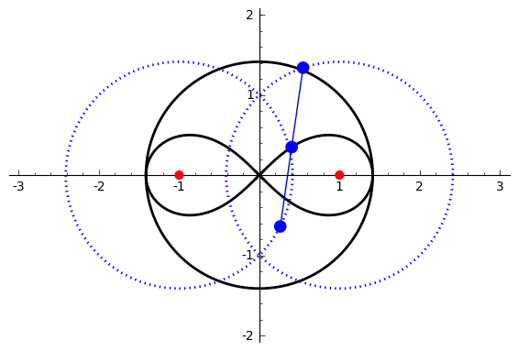
\includegraphics[width=0.5\textwidth]{papers/geradlinig/figures/lemniskate.png}
    \caption{Lemniskate von Bernoulli als Spezialfall der Wattschen Kurve~\cite{watt_curve}.}
    \label{fig:lemniskate}
\end{figure}

Später entwickelte Watt eine modifizierte Version seines Mechanismus,
welcher in Abbildung~\ref{fig:watts_parallel_link} dargestellt ist.
Diesen liess er anschliessend auch patentieren und verbaute ihn in seiner Maschine,
gemäss Abbildung~\ref{fig:watts_engine}.
Diese Konstruktion wird als Parallelbewegungsmechanismus bezeichnet.
Sie war für den praktischen Einsatz besser geeignet 
als die ursprüngliche Ausführung, da sich damit zwei Kolben antreiben liessen.
\begin{figure}
    \centering
    \begin{minipage}{0.32\textwidth}
        \centering
        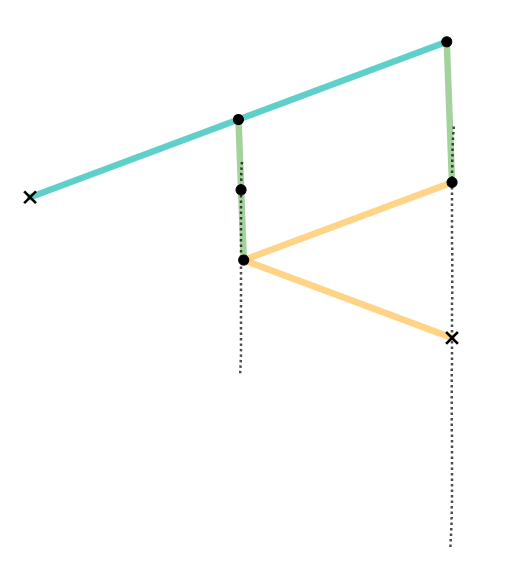
\includegraphics[width=\textwidth]{papers/geradlinig/figures/watts_parallel_linkage1.png}
    \end{minipage}
    \hfill
    \begin{minipage}{0.32\textwidth}
        \centering
        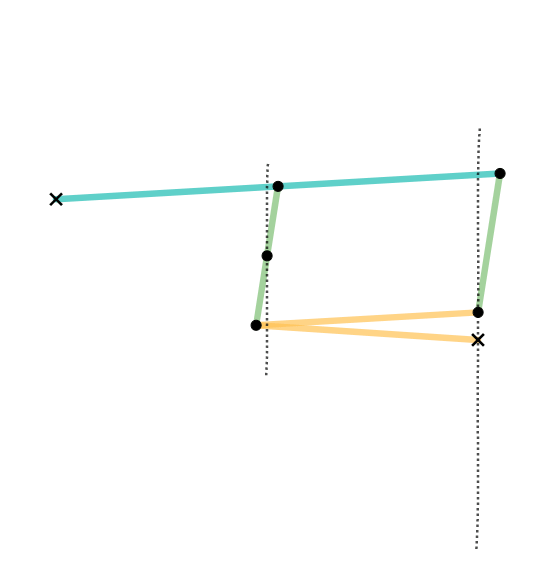
\includegraphics[width=\textwidth]{papers/geradlinig/figures/watts_parallel_linkage2.png}
    \end{minipage}
    \hfill
    \begin{minipage}{0.32\textwidth}
        \centering
        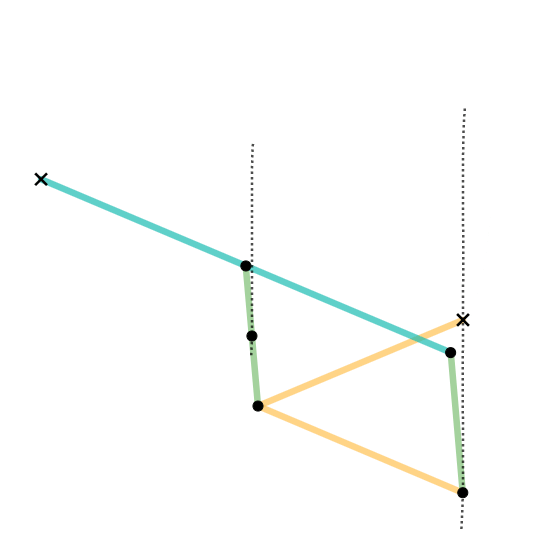
\includegraphics[width=\textwidth]{papers/geradlinig/figures/watts_parallel_linkage3.png}
    \end{minipage}
    \caption{Der Parallelbewegungsmechanismus von Watt~\cite{watt_linkage}.}
    \label{fig:watts_parallel_link}
\end{figure}

Ein weiteres Beispiel ist der Chebyshev-Mechanismus, 
welcher in Abbildung~\ref{fig:chebyshev_link} dargestellt ist.
Dieser besitzt die gleiche Anzahl an Gelenken wie der Watt-Mechanismus, 
verwendet jedoch eine andere Anordnung, 
um eine Rotationsbewegung in eine geradlinige Bewegung umzuwandeln.
Das Verhältnis der gelben Gelenklänge zur blauen beträgt $2.5:1$.
Weitere Mechanismen, welche approximative geradlinige Bewegungen erzeugen, 
sind in~\cite{wiki_straight_line} aufgeführt.
\begin{figure}
    \centering
    \begin{minipage}{0.32\textwidth}
        \centering
        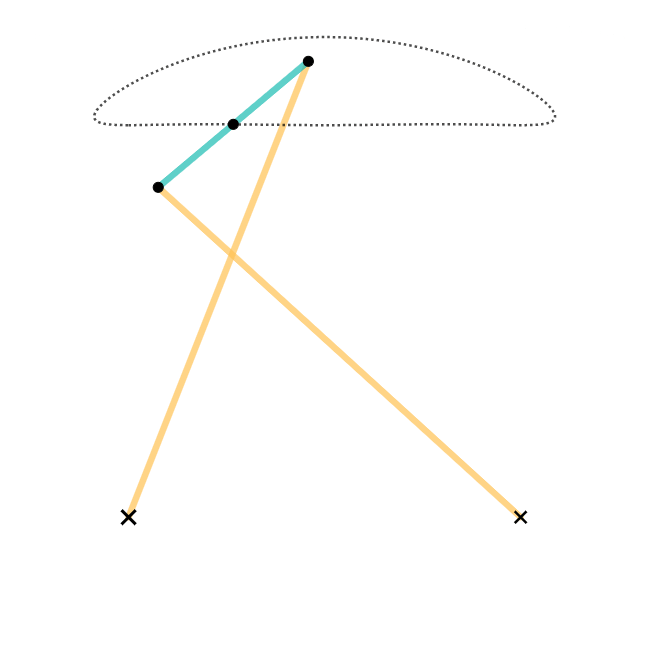
\includegraphics[width=\textwidth]{papers/geradlinig/figures/chebyshev_linkage1.png}
    \end{minipage}
    \hfill
    \begin{minipage}{0.32\textwidth}
        \centering
        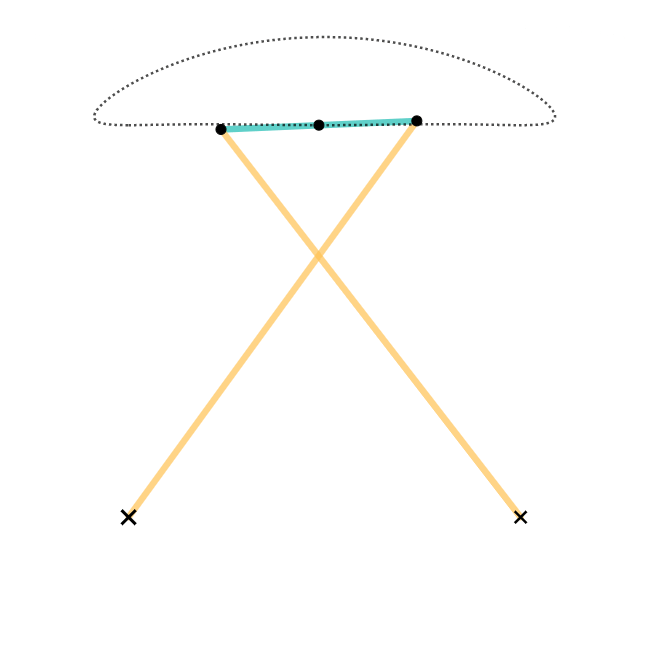
\includegraphics[width=\textwidth]{papers/geradlinig/figures/chebyshev_linkage2.png}
    \end{minipage}
    \hfill
    \begin{minipage}{0.32\textwidth}
        \centering
        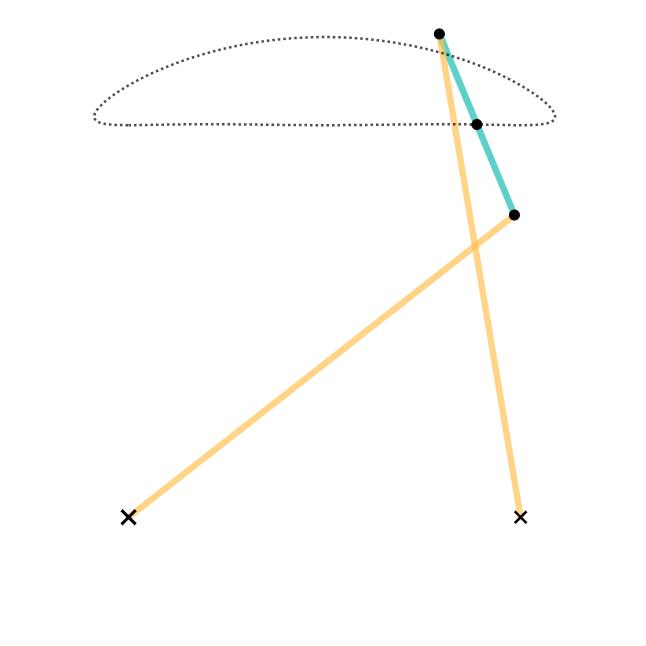
\includegraphics[width=\textwidth]{papers/geradlinig/figures/chebyshev_linkage3.png}
    \end{minipage}
    \caption{Der Mechanismus von Chebyshev~\cite{chebyshev_linkage}.}
    \label{fig:chebyshev_link}
\end{figure}

